\section{Choosing window size}

Nuno in [Tuning Paxos for high-throughput with batching and pipelining] stated that:
\begin{quotation}
A note on the cluster results: In the experiments performed in a cluster environment, batching by itself is enough to achieve the maximum throughput, with pipelining having minimal impact on the results. The reason for this difference is that the latency in a cluster is very low so the leader does not have time to start new instances while waiting for the results of previous instances.
\end{quotation}
This is however false. (At least on HPC cluster.)

During the tests first window size 1÷5 has been tested, showing that the higher window size, the better the results are:\\
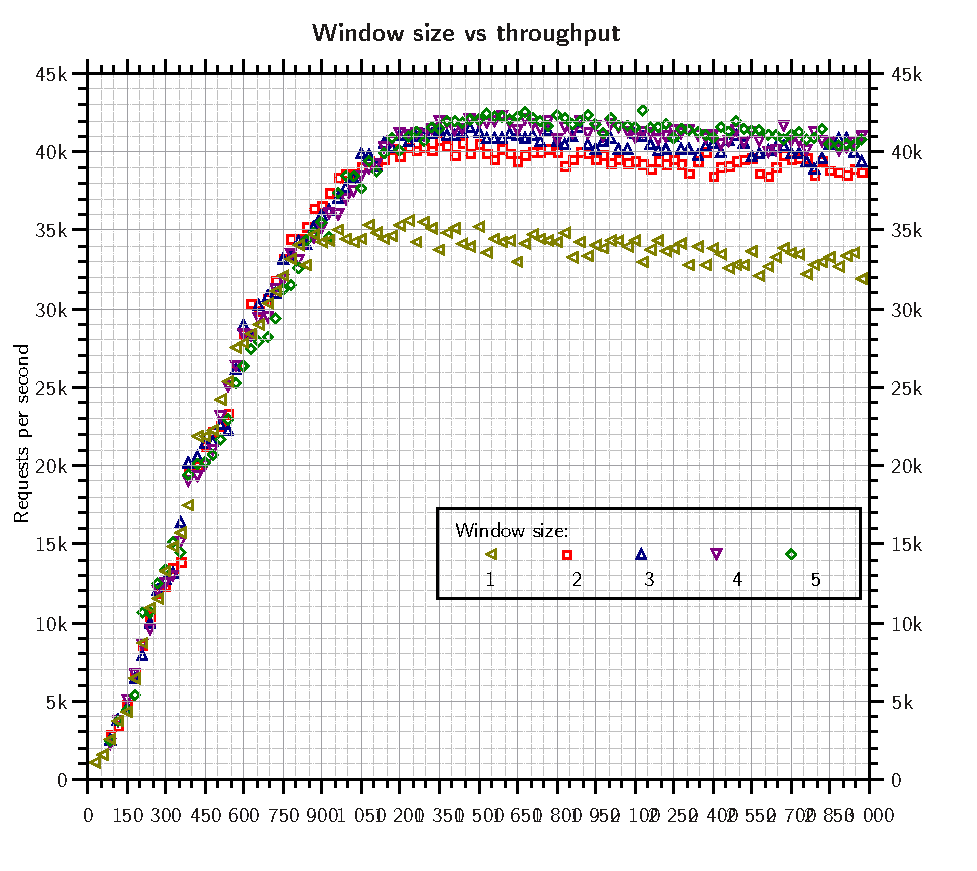
\includegraphics{varia/ws.pdf}

The tests have been continued up to window size 10, as the performance increase stabilized at window size 6 and higher.
To present the results in more readable way, the points represent the gain (in \%) from the worst result at each client count:\\
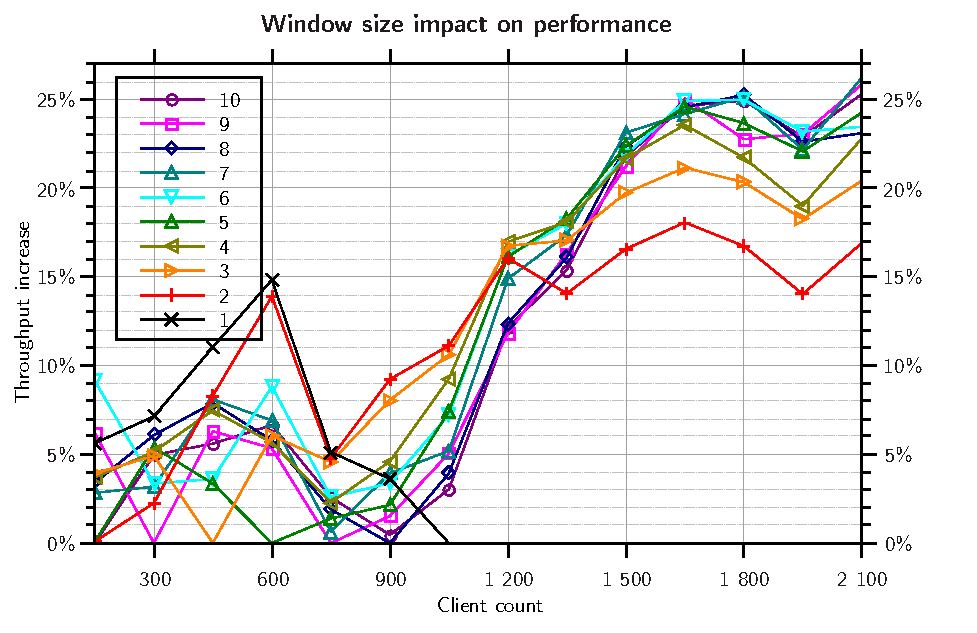
\includegraphics{varia/ws_2d.pdf}

To make the results even more readable (at least for me) the performance gain has been also presented on a 3d plot -- x and y axes represent client count and window size accordingly, while the colour - the brighter the better - represents performance gain:\\
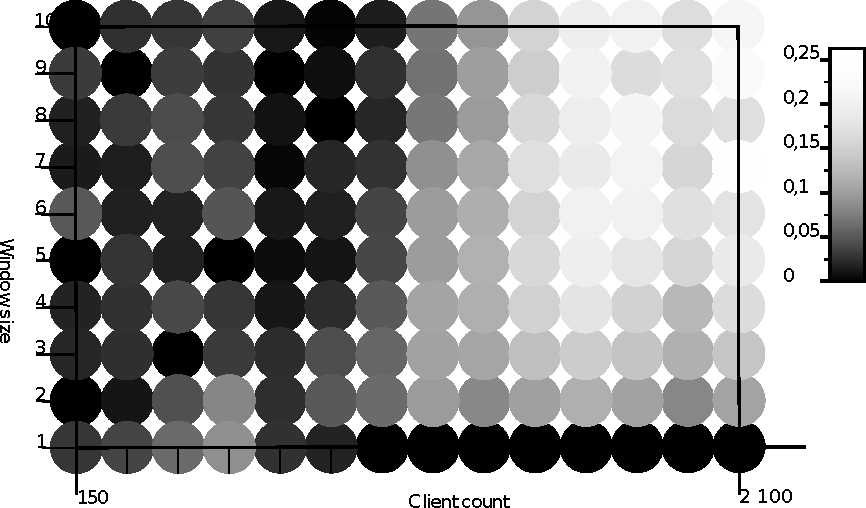
\includegraphics{varia/ws_3d.pdf}

What is not presented on the plots is the variance of the results. As for each client count and window size JPaxos has been run 10 times, except from bare performance also the variance of the performance can be calculated. The results are presented below -- \emph{notice:} the color scale is not linear this time \\
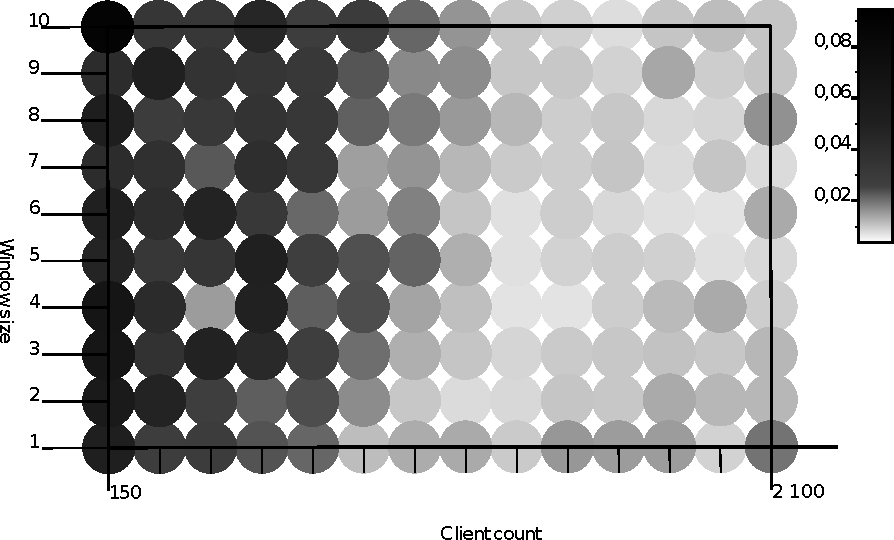
\includegraphics{varia/ws_3d_dev.pdf}

As long as the network is not saturated, the throughput is not stable; after the network becomes the bottleneck, the results are rather stable.

\paragraph{Conclusions}
The window size (and whole pipelining optimisation) is also important on cluster environments, increasing the speed in critical cases by 25\% compared to no pipelining. As long as the network is not saturated, the result stdev is about 5\%, and the gains are in order of 5\% as well. On one hand, this makes choosing right window size hard, on the other -- the performance loss on wrong choice is not big. After saturating the network pipelining increases the performance a lot. Also the stdev drops to 1\%, making the results easier repeatable.

The window size of 6 and higher seems to be the best choice. It is advised to keep the window size as low as possible (due to its negative impact on the speed of recovering from any failures, i.e., view change and recovery). So proper window size for HPC cluster at tests with 1kB requests is six. 
